\PassOptionsToPackage{english}{babel}
\documentclass{report}
\usepackage[utf8]{inputenc}

%\usepackage[english]{babel}
%\usepackage[latin1]{inputenc}
%\usepackage{geometry}
%\usepackage{listings}
\usepackage{caption}
\usepackage{amsmath}
\usepackage{graphics}
\usepackage[T1]{fontenc}
\usepackage{enumitem} %bold enumeration
\usepackage[utf8]{inputenc}
\usepackage[english]{babel}
%\usepackage{pmgraph}
\usepackage{mathrsfs}
\usepackage{floatflt}
\usepackage{multicol}
\usepackage{color,colortbl}
% \usepackage[pdftex]{graphicx}
\usepackage[normalem]{ulem}
\usepackage[colorlinks,urlcolor=blue, linkcolor=blue]{hyperref}
\usepackage{epstopdf}
\usepackage{wrapfig}
\usepackage{multirow}
%% Sets page size and margins
\usepackage[a4paper,top=3cm,bottom=2cm,left=3cm,right=3cm,marginparwidth=1.75cm]{geometry}
%% Useful packages
\usepackage[colorinlistoftodos]{todonotes}
\usepackage{xymtex}
\usepackage{fancyhdr}
\usepackage{epstopdf}
\usepackage{indentfirst} \geometry{verbose,a4paper,tmargin=3cm,bmargin=3cm,lmargin=1.0cm,rmargin=2.0cm}
\setlength{\parindent}{0pt}
 \graphicspath{C:/Users/Anton/Desktop/ETH_books/CV/CV-Lab-Model-Fitting/CV-Lab-Model-Fitting/src/epipolar_geometry/res}
\begin{document}
\large
Report of Anton Maksimov (antonma, 16-952-137), Task 7 "Structure from motion"\\
 on ETHZ course "Computer Vision".\\
\rule{\linewidth}{1pt}
%%%%%%%%%%%%%%%%%%%%%%%%%%%%%%%%%%%%%%%%%%%%%%%%%%%%%%%%%   1
	\textbf{1.} Using 8--point RANSAC we estimate fundamental matrix $F$ of the first pair of images (the first and the last), matches are extracted with SIFT (RANSAC tthreshold $10^{-4}$). After that we compute essential matrix as $E = K^\top F K$ using provided camera matrix $K$. We obtain projection matrix using \texttt{decomposeE.m}. Then we triangulate corresponding inliers (with \texttt{linearTriangulation.m}), which were calibrated on cameras multiplying $K^{-1}\cdot$ and use as the identity projection matrix for the first image points and obtained one for the last image points.
	
	\begin{figure}[h]
		\begin{center}
			\begin{minipage}[h]{0.45\linewidth}
				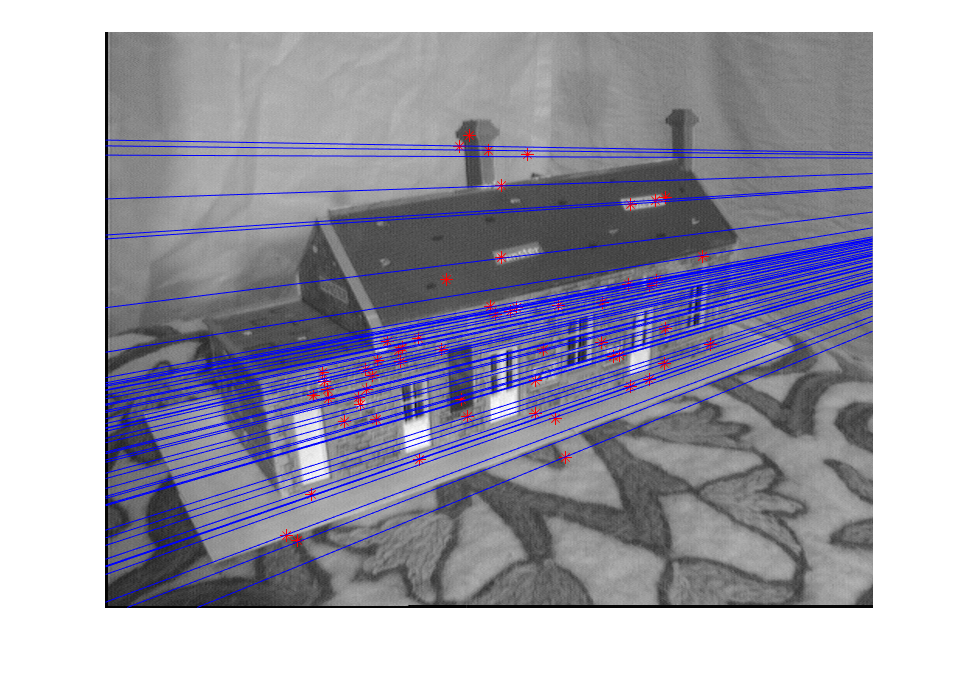
\includegraphics[width=1\linewidth, trim = {2cm 1cm 2cm 1cm}, clip]{C:/Users/Anton/Desktop/ETH_books/CV/Exercise7/results/epi1}
			\end{minipage}
			\hfill
			\begin{minipage}[h]{0.45\linewidth}
			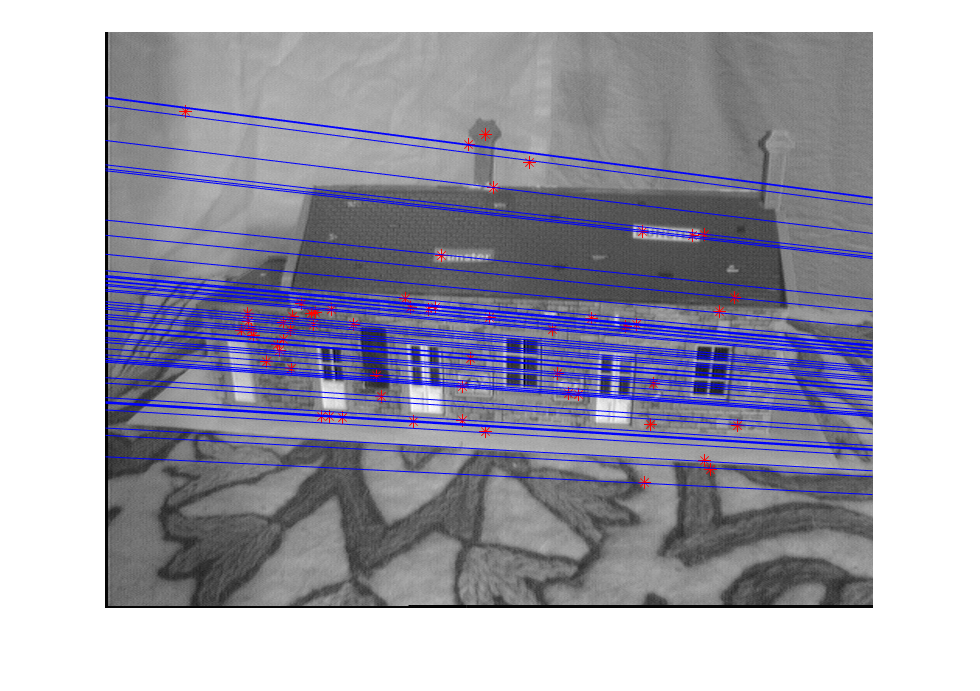
\includegraphics[width=1\linewidth, trim = {2cm 1cm 2cm 1cm}, clip]{C:/Users/Anton/Desktop/ETH_books/CV/Exercise7/results/epi2}
		\end{minipage}
		\caption{Epipolar lines corresponding to fundamental matrix calculated from the first and the last images. Relative position of the first camera is almost orthogonal to the view of the second, so the epipolar lines are almost parallel. Epipolar lines on the first image intersects at the adequate point --- position of the second camera. To plot epipolar lines we used code from one of the previous tasks.}
	\end{center}
\end{figure}
	\begin{figure}[h]
		\begin{center}
			\begin{minipage}[h]{0.9\linewidth}
				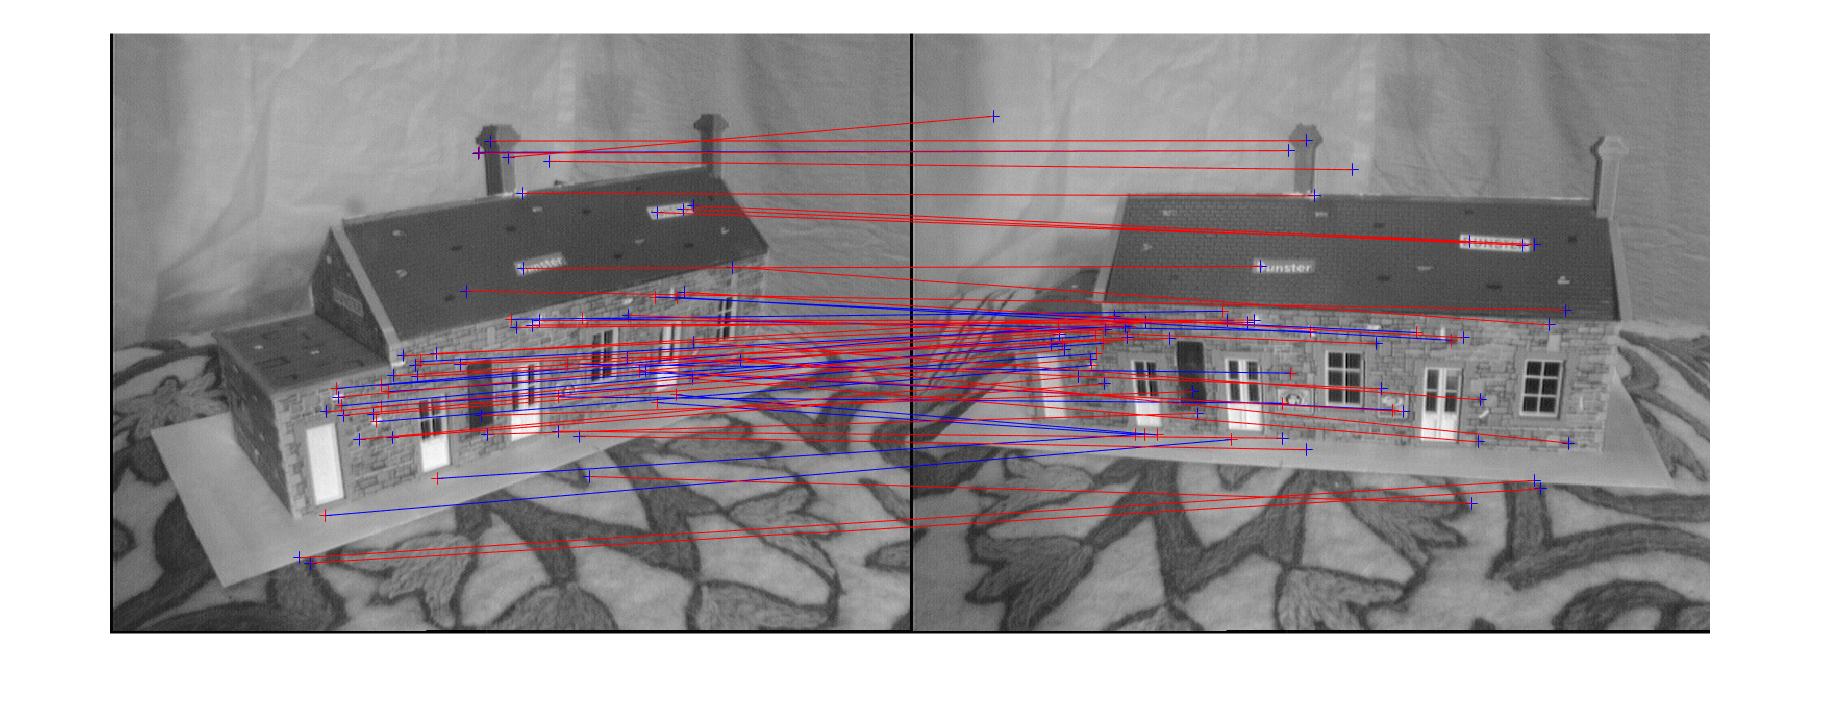
\includegraphics[width=1\linewidth, trim = {2cm 1cm 2cm 1cm}, clip]{C:/Users/Anton/Desktop/ETH_books/CV/Exercise7/results/20}
				\caption{Initial search of matches between the first and the last (fifth) images using 8--point RANSAC, red lines show outliers, blue --- inliers.}
			\end{minipage}
	\end{center}
\end{figure}
%%%%%%%%%%%%%%%%%%%%%%%%%%%%%%%%%%%%%%%%%%%%%%%%%%%%%%%%%%%%%%%%%%
\newpage
\textbf{2--3.} Using included function \texttt{ransacfitprojmatrix.m} (which is 6-point RANSAC with included 6-point DLT in order to have an error measure as reprojection error) we obtain projection matrices for other views relative to the first view. Similarly to previous we obtain triangulated 3D-point and plot them in the end. All this is implemented as a function \texttt{addView} which is called for every new view (fig. 3--6, resulting points and cameras at fig. 7).
	\begin{figure}[h]
		\begin{center}
	\begin{minipage}[h]{0.9\linewidth}
		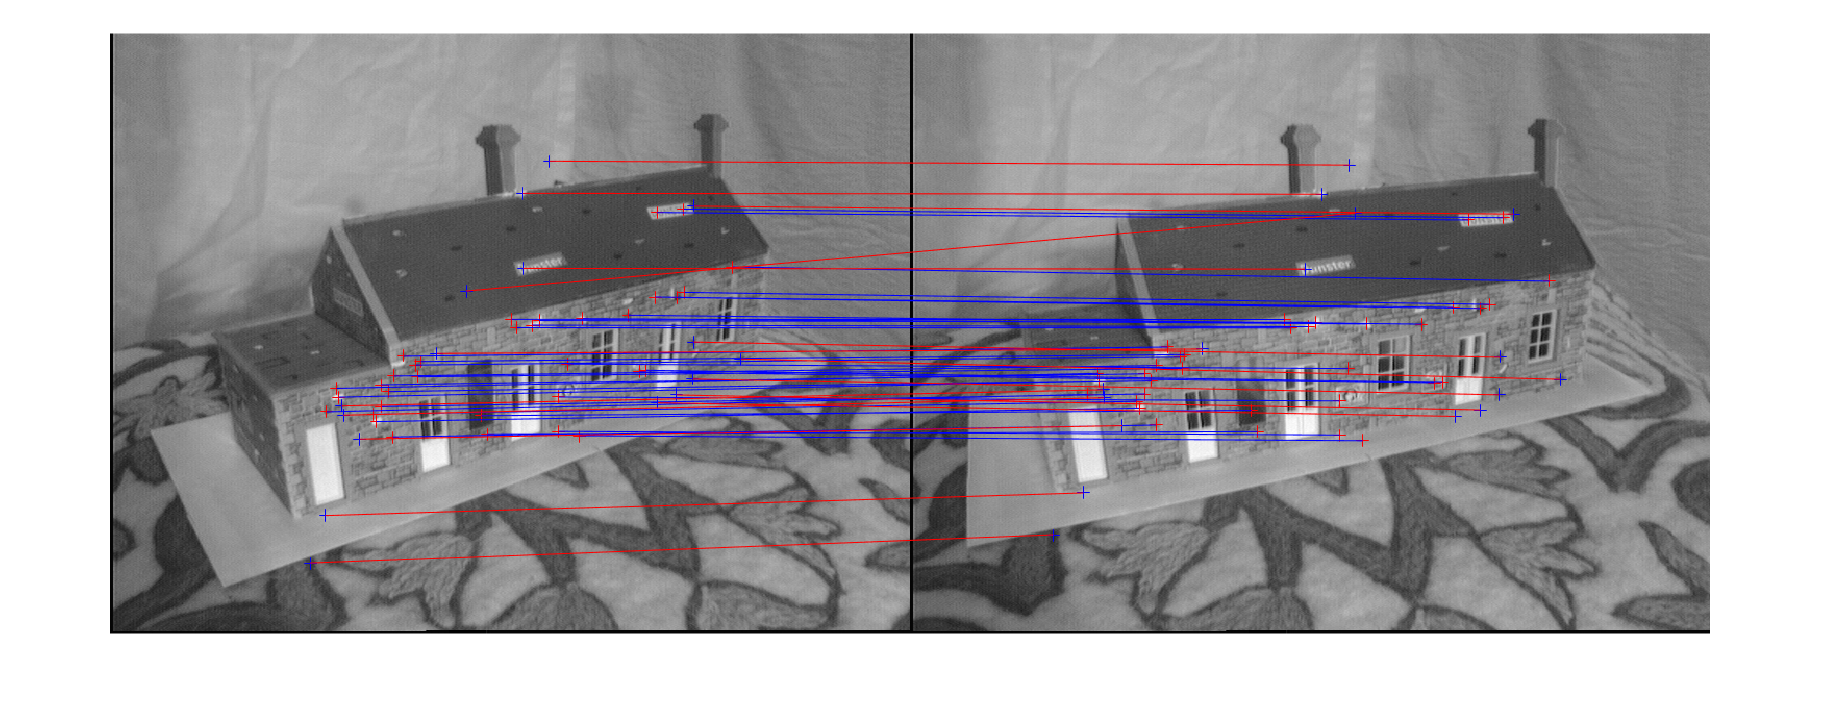
\includegraphics[width=1\linewidth, trim = {2cm 1cm 2cm 1cm}, clip]{C:/Users/Anton/Desktop/ETH_books/CV/Exercise7/results/21}
		\caption{Between first and second images.}
	\end{minipage}
	\vfill
	\begin{minipage}[h]{0.9\linewidth}
		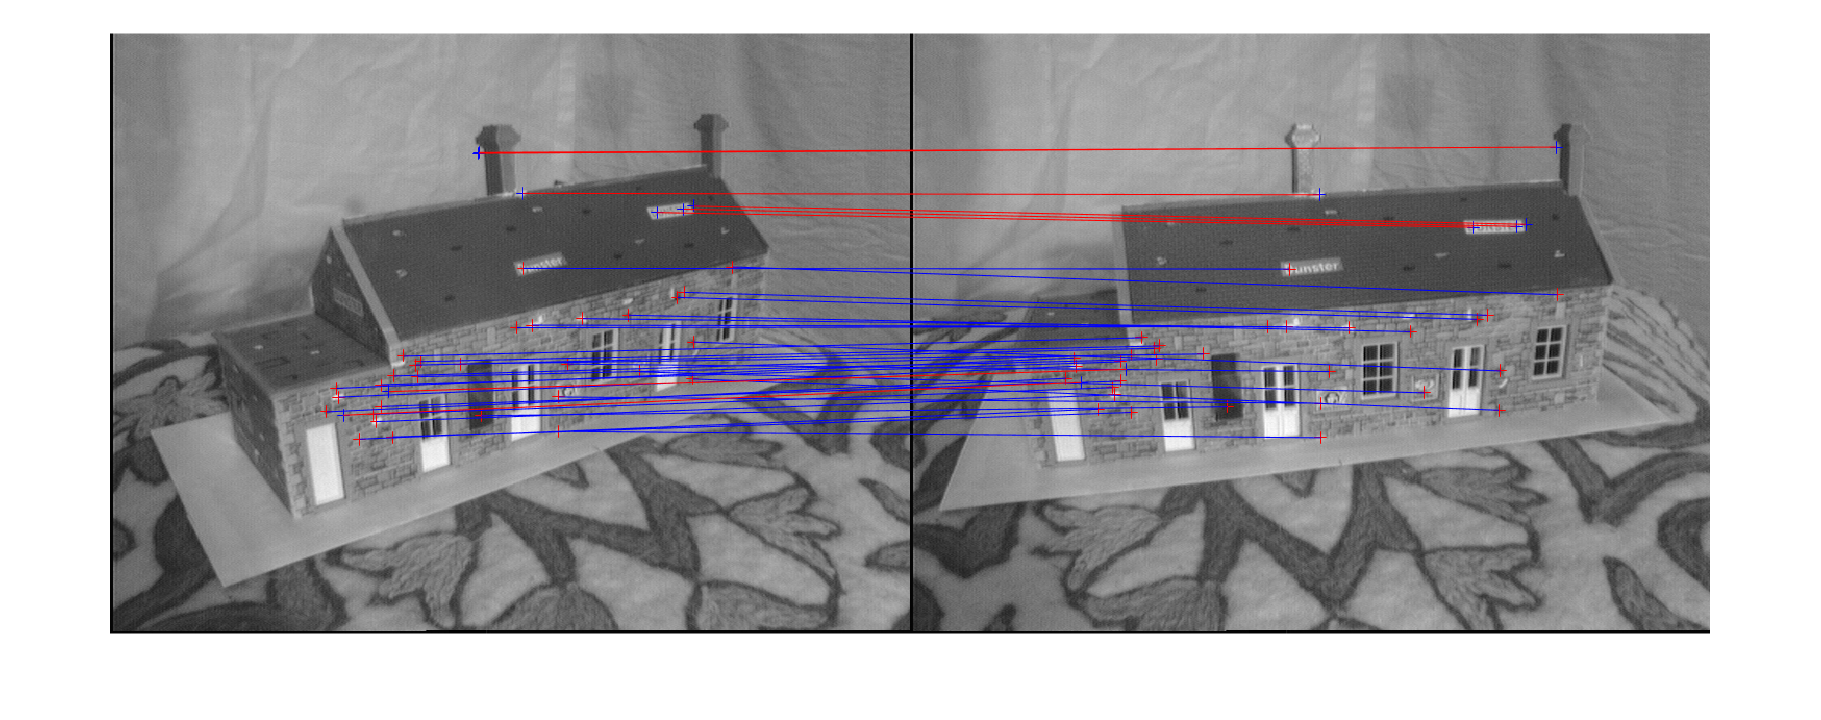
\includegraphics[width=1\linewidth, trim = {2cm 1cm 2cm 1cm}, clip]{C:/Users/Anton/Desktop/ETH_books/CV/Exercise7/results/22}
		\caption{Between first and third images.}
	\end{minipage}
	\vfill
	\begin{minipage}[h]{0.9\linewidth}
		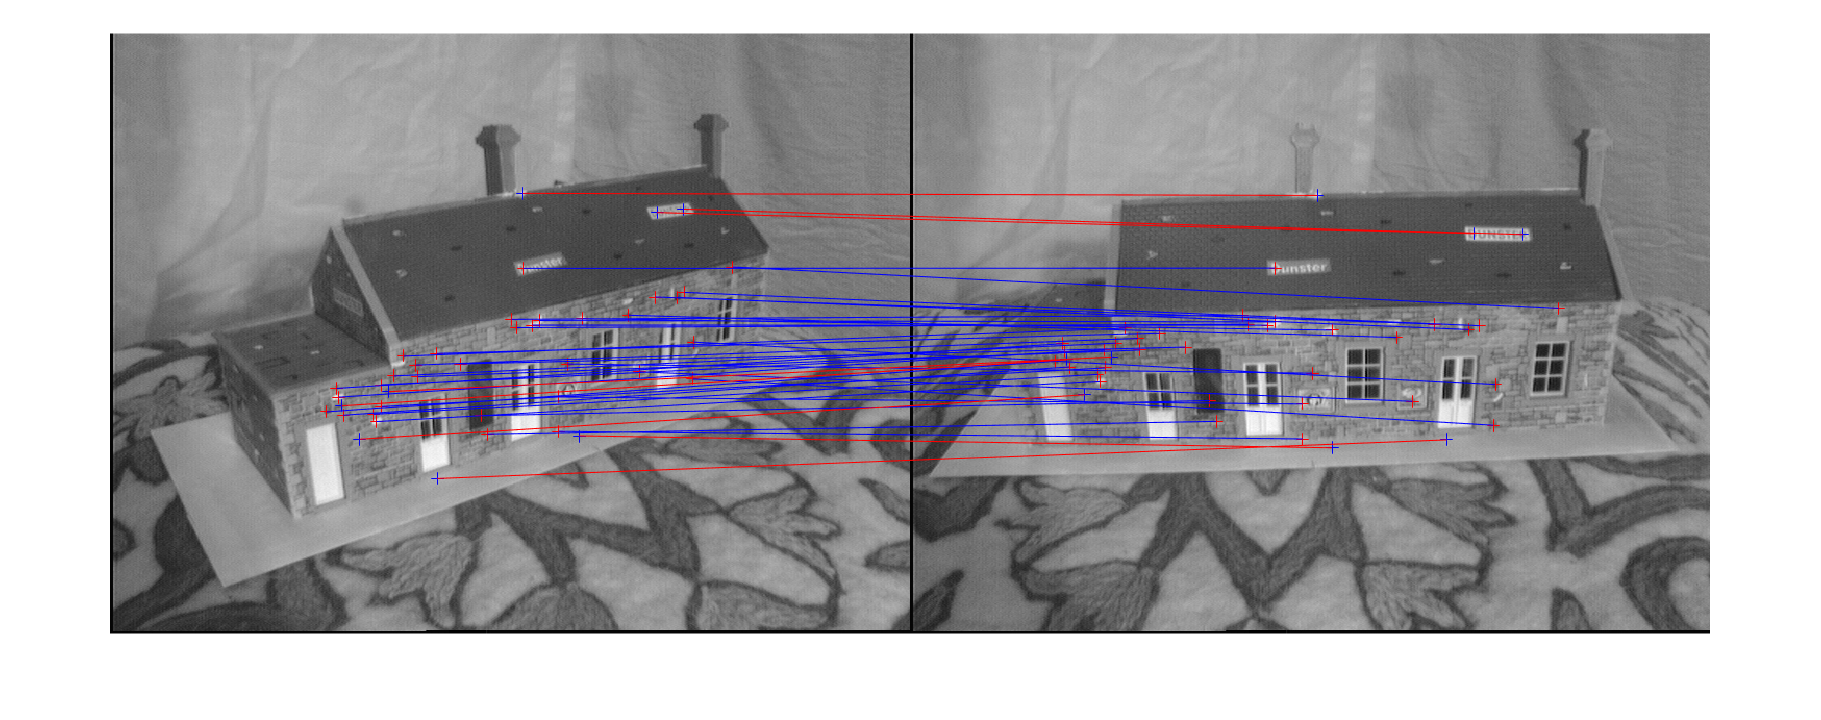
\includegraphics[width=1\linewidth, trim = {2cm 1cm 2cm 1cm}, clip]{C:/Users/Anton/Desktop/ETH_books/CV/Exercise7/results/23}
		\caption{Between first and fourth images.}
	\end{minipage}
		\end{center}
	\caption{Matches between images obtained using using 6--point RANSAC and with selection of inliers using 6--point DLT (filtering using corresponding reprojection error), red lines show outliers, blue --- inliers.}
	\end{figure}


\textbf{4.} 
In order to get dense reconstruction we use code from the previous task6 adapted for this task. We change almost only \texttt{exercise6.m} file in \texttt{dispairity} folder, which in called from \texttt{exercise8} in order to obtain dispairity map and rectified images (using graph-cut as the best in quality method from two used in task6), which are then triangulated to produce 3D-image using as projection matrices ones obtained from the obligatory part of the task. (fig. 8)
	\begin{figure}[h]
	\begin{center}
		\begin{minipage}[h]{0.45\linewidth}
			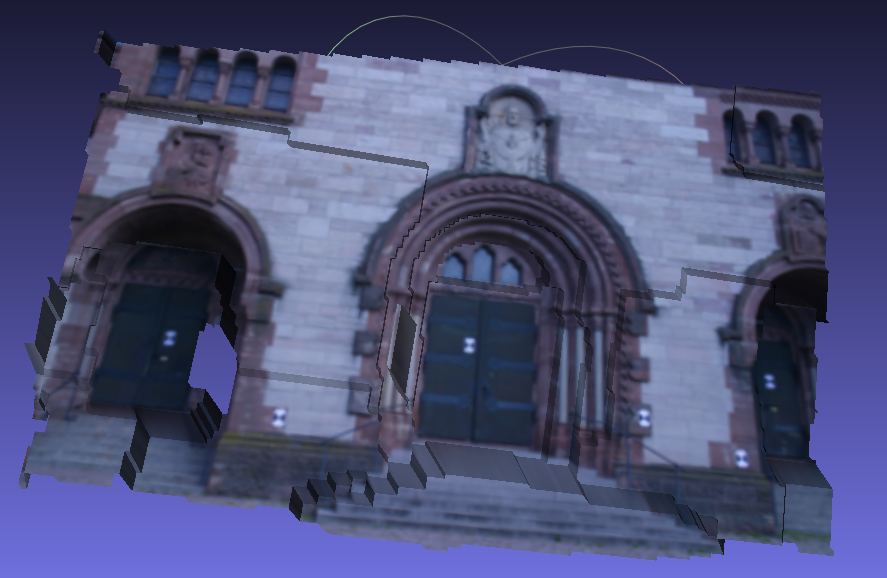
\includegraphics[width=1\linewidth, trim = {15cm 3cm 17cm 5cm}, clip]{C:/Users/Anton/Desktop/ETH_books/CV/Exercise7/results/1}
		\end{minipage}
		\hfill
		\begin{minipage}[h]{0.45\linewidth}
			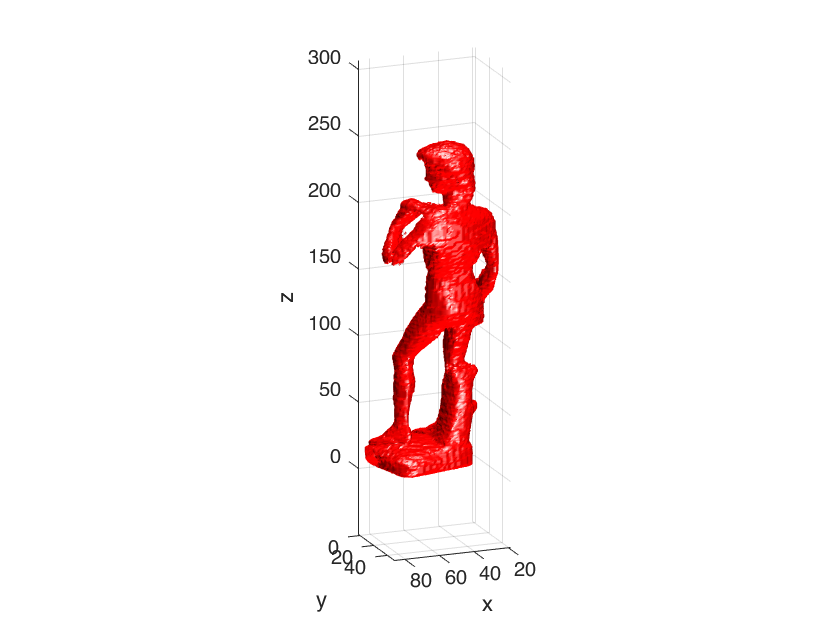
\includegraphics[width=1\linewidth, trim = {15cm 3cm 17cm 5cm}, clip]{C:/Users/Anton/Desktop/ETH_books/CV/Exercise7/results/2}
		\end{minipage}
		\caption{Triangulated 3D-points (sparse reconstruction)  and camera poses extracted from images (red --- from the first triangulation during initialization). Blue axes show depth of the camera (direction of view from the camera origin), and this corresponds to the true their arrangement (fan--like). There are much less points from other than the first views, and some are outliers, which could be caused by non-ideality of RANSAC + use of points which are at the background of house.}
	\end{center}
\end{figure}

\begin{figure}[h]
\begin{center}
	\begin{minipage}[h]{0.6\linewidth}
		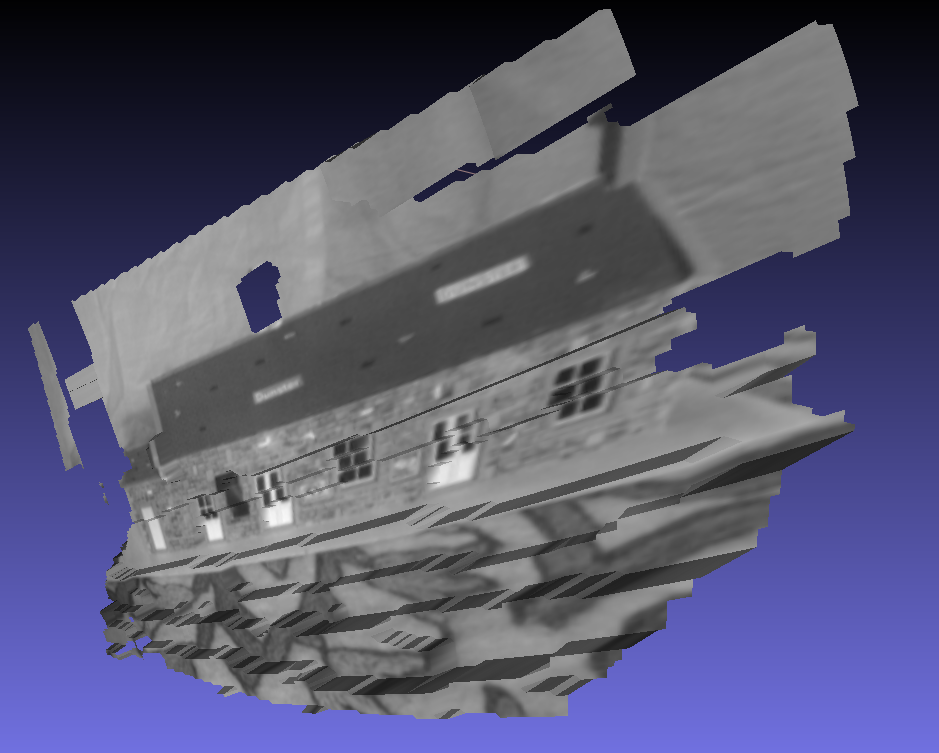
\includegraphics[width=1\linewidth]{C:/Users/Anton/Desktop/ETH_books/CV/Exercise7/results/3D-3}		
	\end{minipage}
\hfill
\begin{minipage}[h]{0.37\linewidth}
	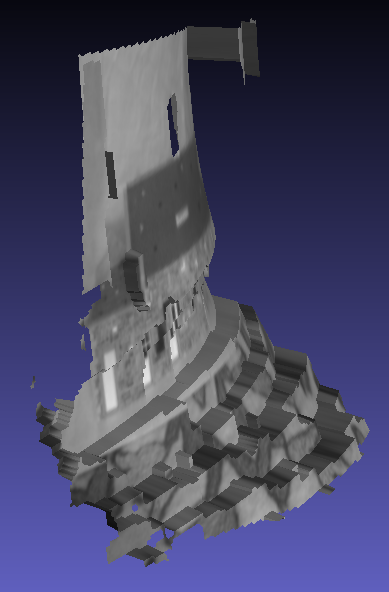
\includegraphics[width=1\linewidth]{C:/Users/Anton/Desktop/ETH_books/CV/Exercise7/results/3D-2}
\end{minipage}
\caption{Dense 3D-reconstruction using the previous lab pipeline (rectification, graph-cut for dispairity, triangulation using projection matrices, which were obtained using this lab results). A little <<steppy>, but shows right change in depth (floor is closer, house is in the middle and backround is deeper). Steps could be better smoothed when changing parameters of graph-cut and using full-scale image (was used window size 20 on the 0.5 scale). As we have grayscale image, we assigned the same grayscale values for every RGB component.}
\end{center}
\end{figure}
\newpage
%%%%%%%%%%%%%%%%%%%%%%%%%%%%%%%%%%%%%%%%%%%%%%%%%%%%%%%%%   2
\end{document}